\documentclass[../notes.tex]{subfiles}

\pagestyle{main}
\renewcommand{\chaptermark}[1]{\markboth{\chaptername\ \thechapter\ (#1)}{}}
\stepcounter{chapter}

\begin{document}




\chapter{???}
\section{Separable ODEs}
\begin{itemize}
    \item \marginnote{10/3:}Do not sit on the left side of the classroom: The sun sucks!
    \item \textbf{Separable} (ODE): An ODE of the form
    \begin{equation*}
        \dv{y}{t} = f(t)g(y)
    \end{equation*}
    where $y$ is a real\footnote{We'll deal with complex functions later.}, unknown, scalar function of $t$.
    \item Solving separable ODEs: Formally, evaluate
    \begin{equation*}
        \int\frac{\dd{y}}{g(y)} = \int f(t)\dd{t}
    \end{equation*}
    \item Rearrange the initial separable ODE to $\dv*{y}{t}\cdot 1/g=f$ and invoke the law of composite differentiation to get
    \begin{equation*}
        \dv{t}\left[ \int_{y_0}^{y(t)}\frac{\dd{w}}{g(w)}-\int_{t_0}^tf(\tau)\dd{\tau} \right] = 0
    \end{equation*}
    \item It follows that
    \begin{equation*}
        \int_{y_0}^{y(t)}\frac{\dd{w}}{g(w)} = \int_{t_0}^tf(\tau)\dd{\tau}
    \end{equation*}
    \item Examples:
    \begin{enumerate}
        \item Exponential growth.
        \begin{itemize}
            \item We have that
            \begin{equation*}
                \dv{y}{t} = ky
            \end{equation*}
            for $k>0$ and $y(0)=y_0>0$.
            \item The solution is
            \begin{align*}
                \frac{1}{y}\cdot\dv{y}{t} &= k\\
                \log y(t)-\log y_0 &= kt\\
                y(t) &= y_0\e[kt]
            \end{align*}
        \end{itemize}
        \item Logistic growth.
        \begin{itemize}
            \item We have that
            \begin{equation*}
                \dv{y}{t} = ky\left( 1-\frac{y}{M} \right)
            \end{equation*}
            for $k,M>0$ and $y(0)=y_0>0$.
            \item The solution is
            \begin{align*}
                \frac{M\dd{y}}{y(M-y)} &= k\dd{t}\\
                \log\frac{y}{M-y}-\log\frac{y_0}{M-y_0} &= kt\\
                \frac{y(M-y_0)}{y_0(M-y)} &= \e[kt]\\
                y\cdot\frac{M-y_0}{y_0} &= (M-y)\e[kt]\\
                y\cdot\frac{M-y_0}{y_0}+y\e[kt] &= M\e[kt]\\
                y\left( \frac{M-y_0}{y_0}+\e[kt] \right) &= M\e[kt]\\
                y\left( \frac{M-y_0+y_0\e[kt]}{y_0} \right) &= M\e[kt]\\
                y\left( \frac{M+y_0(\e[kt]-1)}{y_0} \right) &= M\e[kt]\\
                y(t) &= \frac{My_0\e[kt]}{M+y_0(\e[kt]-1)}
            \end{align*}
            \item Sketches the graph of logistic growth and discusses the turning point (for which there is a formula; zero of the second derivative) as well as general trends.
            \item If $y_0<0$, the solution is not physically meaningful, but it is mathematically insightful.
            \begin{itemize}
                \item When we integrate, the arguments of our logarithms now have absolute values.
                \begin{equation*}
                    \log\left| \frac{y}{M-y} \right|-\log\left| \frac{y_0}{M-y_0} \right| = kt
                \end{equation*}
                \item We need to make sure that the denominator of the final logistic form is never equal to zero, but now that $y_0$ is negative, as $t$ increases, the denominator will approach zero exponentially. It reaches zero when
                \begin{align*}
                    M+y_0(\e[kt]-1) &= 0\\
                    \e[kt] &= -\frac{M}{y_0}+1
                \end{align*}
                In other words, $t_\text{max}=(1/k)\log(1-M/y_0)$ because when $t=t_\text{max}$, the equation blows up.
                \item This is an example of \textbf{finite lifespan}.
            \end{itemize}
            \item If $y_0>M$, then you will exponentially decrease to $M$.
        \end{itemize}
        \item Lotka-Volterra predator-prey model.
        \begin{itemize}
            \item We have that
            \begin{align*}
                r' &= k_1r-awr&
                w' &= -k_2w+bwr
            \end{align*}
            where $r$ is rabbits and $w$ is wolves.
            \item We can rename the variables to
            \begin{equation*}
                \begin{cases}
                    x' = Ax-Bxy\\
                    y' = -Cy+Dxy
                \end{cases}
            \end{equation*}
            \item Dividing, we get
            \begin{align*}
                \frac{x'}{y'} &= \frac{Ax-Bxy}{-Cy+Dxy}\\
                \frac{By-A}{y}y'+\frac{Dx-C}{x}x' &= 0
            \end{align*}
            \item Use the fact that $x,y$ are independent variables, so both terms in the above equation are equal to zero?
            \item Invoke the law of composite differentiation twice and, from the above, know that $0+0=0$, so we can add the two solutions:
            \begin{align*}
                \dv{t}(By(t)-A\log y(t))+\dv{t}(Dx(t)-C\log x(t)) &= 0\\
                By(t)-A\log y(t)+Dx(t)-C\log x(t) &= E
            \end{align*}
            \item Sketches some of the trajectories (they're all closed curves in the $xy$-plane).
            \begin{figure}[h!]
                \centering
                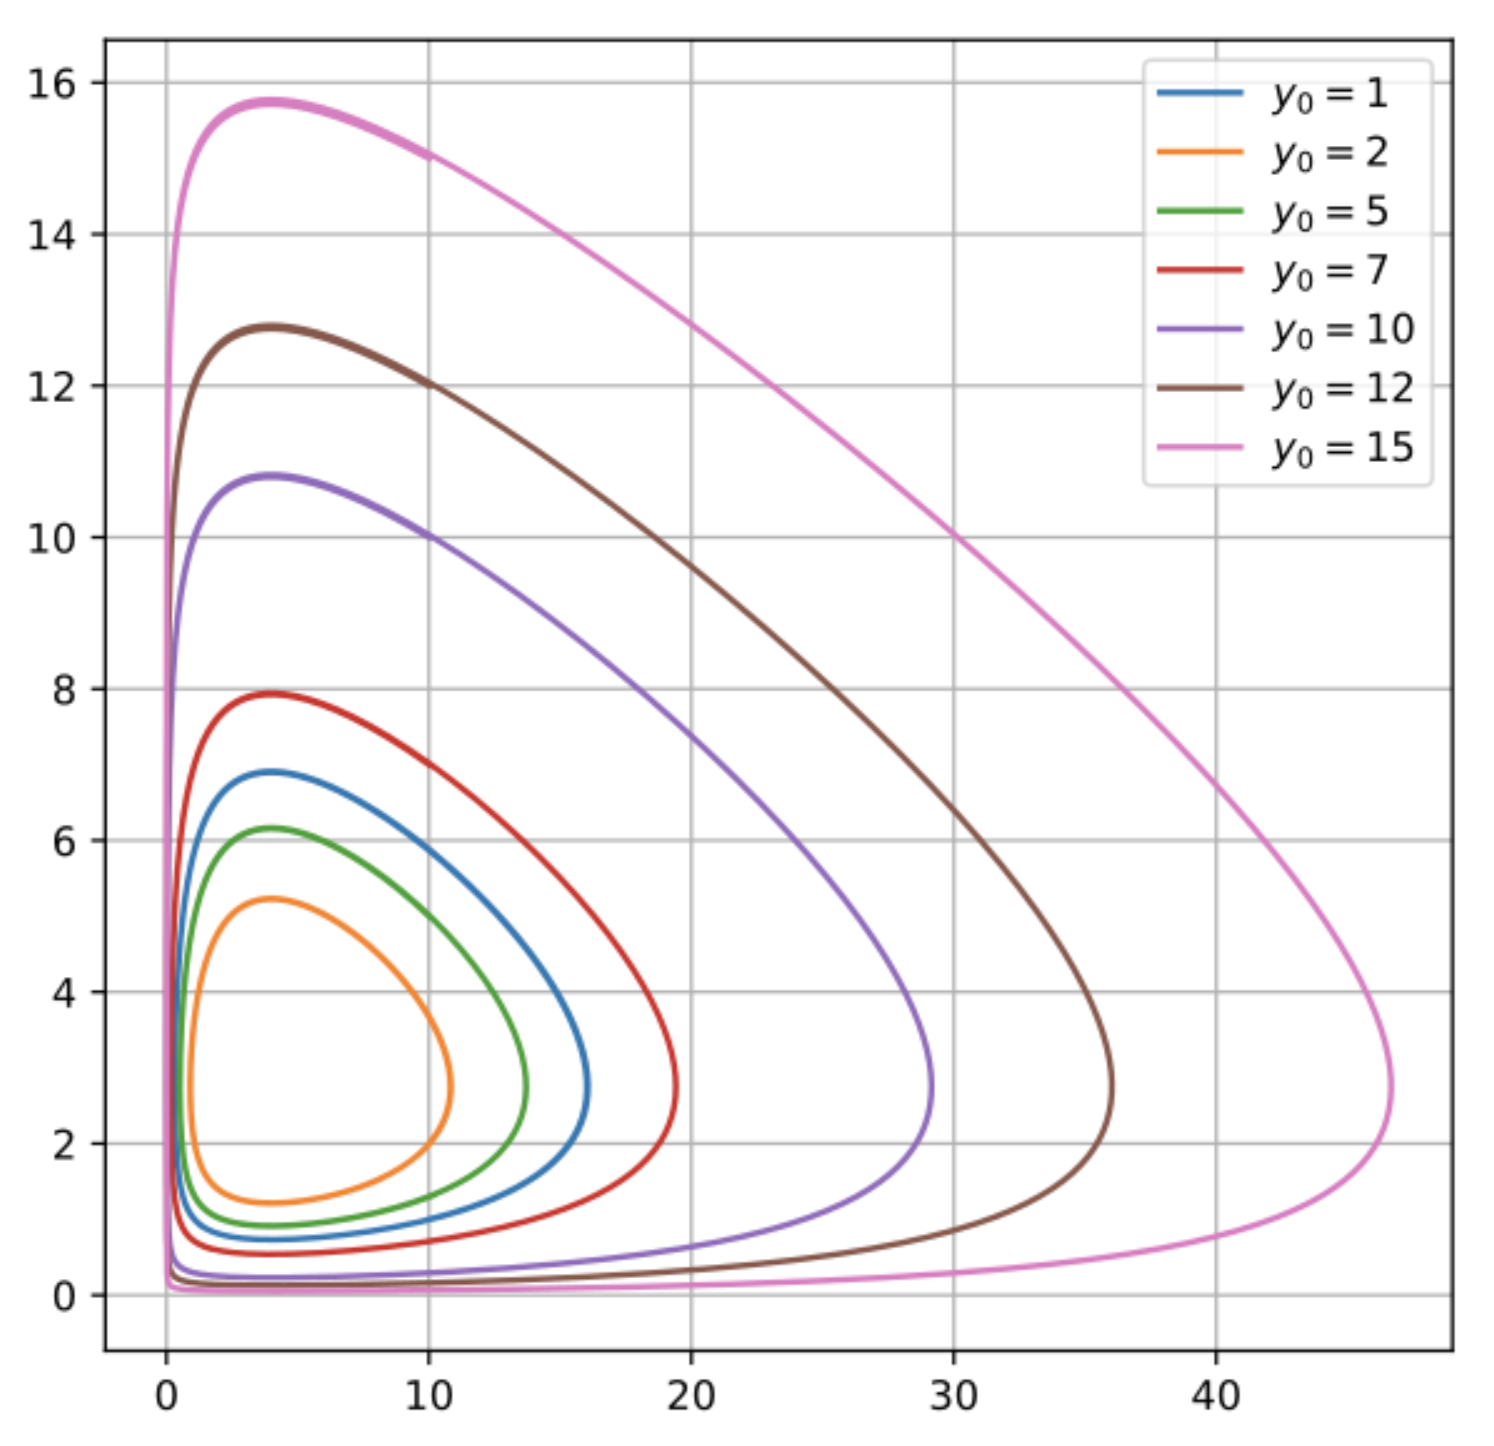
\includegraphics[width=0.4\linewidth]{../ExtFiles/LotkaVolteraSolns.png}
                \caption{Lotka-Volterra solution curves.}
                \label{fig:LotkaVolteraSolns}
            \end{figure}
            \item Properties of the curves:
            \begin{itemize}
                \item The implicit relation which determines them: By the implicit function theorem, the $y$ derivative of the LHS is $B-A/y$ and the $x$-derivative of the LHS is $D-C/x$. When the partial derivatives are equal to zero, $(C/D,A/B)$ becomes interesting. Turning points happen when the $y$-coordinate is $A/B$ or the $x$-coordinate is $C/D$.
            \end{itemize}
        \end{itemize}
    \end{enumerate}
    \item \textbf{Finite lifespan}: Even if the RHS of $\dv*{y}{t}=f(t,y)$ is very regular, the solution can still blow up at some finite time.
    \item Consider the following variation on the E-L equation from the Brachistochrone problem.
    \begin{equation*}
        \dv{y}{x} = \sqrt{\frac{B-y}{y}}
    \end{equation*}
    \begin{itemize}
        \item Finding the \textbf{primitives}.
        \begin{itemize}
            \item What are these "primitives" Shao keeps talking about?
        \end{itemize}
        \item We should have
        \begin{equation*}
            \int\sqrt{\frac{y}{B-y}}\dd{y} = x
        \end{equation*}
        \item Change of variables: $y=B\sin^2\phi$ and $\dd{y}=2B\cos\phi\sin\phi\dd{\phi}$. Thus,
        \begin{equation*}
            \int\sqrt{\frac{y}{B-y}}\dd{y} = \int\frac{\sin\phi}{\cos\phi}\cdot 2B\cos\phi\sin\phi\dd{\phi}
            = 2B\int\sin^2\phi\dd{\phi}
        \end{equation*}
        \item The solution is
        \begin{equation*}
            \begin{cases}
                x = B\phi-\frac{B}{2}\sin(2\phi)+C\\
                y = B\sin^2\phi
            \end{cases}
        \end{equation*}
        \begin{itemize}
            \item This is a parameterization of a cycloid.
        \end{itemize}
    \end{itemize}
    \item Later in the week, we will do the SHM, the pendulum, the Kepler 2-body problem, and the Michaelis-Menten equation.
    \item Separable ODEs are a subset of ODEs of \textbf{exact form}.
    \item ODEs of exact form are of the form
    \begin{equation*}
        g(x,y)\dv{y}{x}+f(x,y) = 0
    \end{equation*}
    where for some $F(x,y)$, $g=\pdv*{F}{y}$, $f=\pdv*{F}{x}$, and partials commute. Equivalently,
    \begin{equation*}
        \pdv{g}{x} = \pdv{f}{y}
    \end{equation*}
    is our necessary and sufficient condition.
    \item By the law of composite differentiation,
    \begin{align*}
        \dv{x}\left[ F(x,y(x)) \right] &= \pdv{F}{x}(x,y(x))+\pdv{F}{y}(x,y(x))\cdot y'(x)\\
        &= f(x,y(x))+g(x,y(x))y'(x)\\
        &= 0
    \end{align*}
    \begin{itemize}
        \item We solve these with an integrating factor $\mu\neq 0$ such that $(\mu g,\mu f)$ satisfy the constraint.
    \end{itemize}
\end{itemize}




\end{document}